

\begin{frame}{Introduction}
  \begin{block}{Recent Many-Core Architectures}
    \begin{itemize}
     \item High FLOP/Watt ratio
     \item High memory bandwidth
     \item Attached via PCI-Express
    \end{itemize}
\vspace*{1cm}
  \end{block}

   \begin{minipage}{0.3\textwidth}
    \begin{center}
     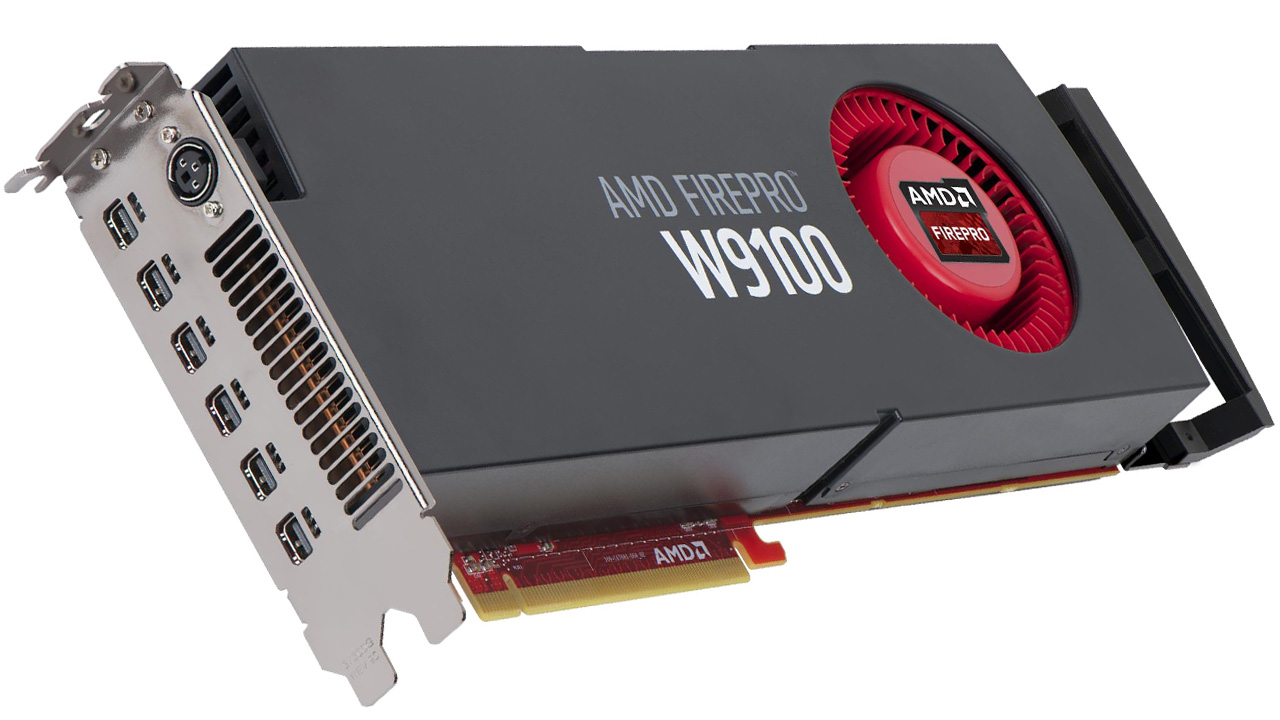
\includegraphics[width=0.99\textwidth]{figures/w9100.jpg} \\ AMD FirePro W9100 \\ 320 GB/sec
    \end{center}
   \end{minipage}
   \hspace{0.2cm}
%
   \begin{minipage}{0.3\textwidth}
    \begin{center}
     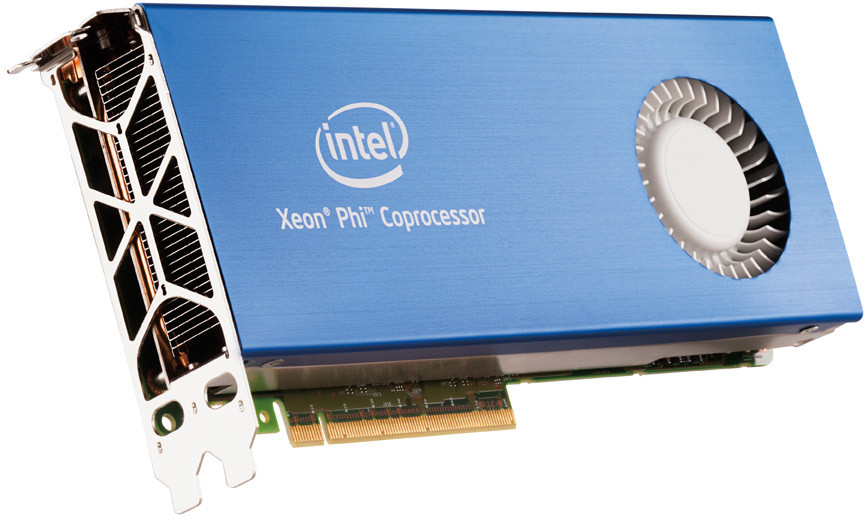
\includegraphics[width=0.92\textwidth]{figures/xeon-phi.jpg} \\ INTEL Xeon Phi \\ 320 (220?) GB/sec
    \end{center}
   \end{minipage}
   \hspace{0.2cm}
%
   \begin{minipage}{0.3\textwidth}
    \begin{center}
     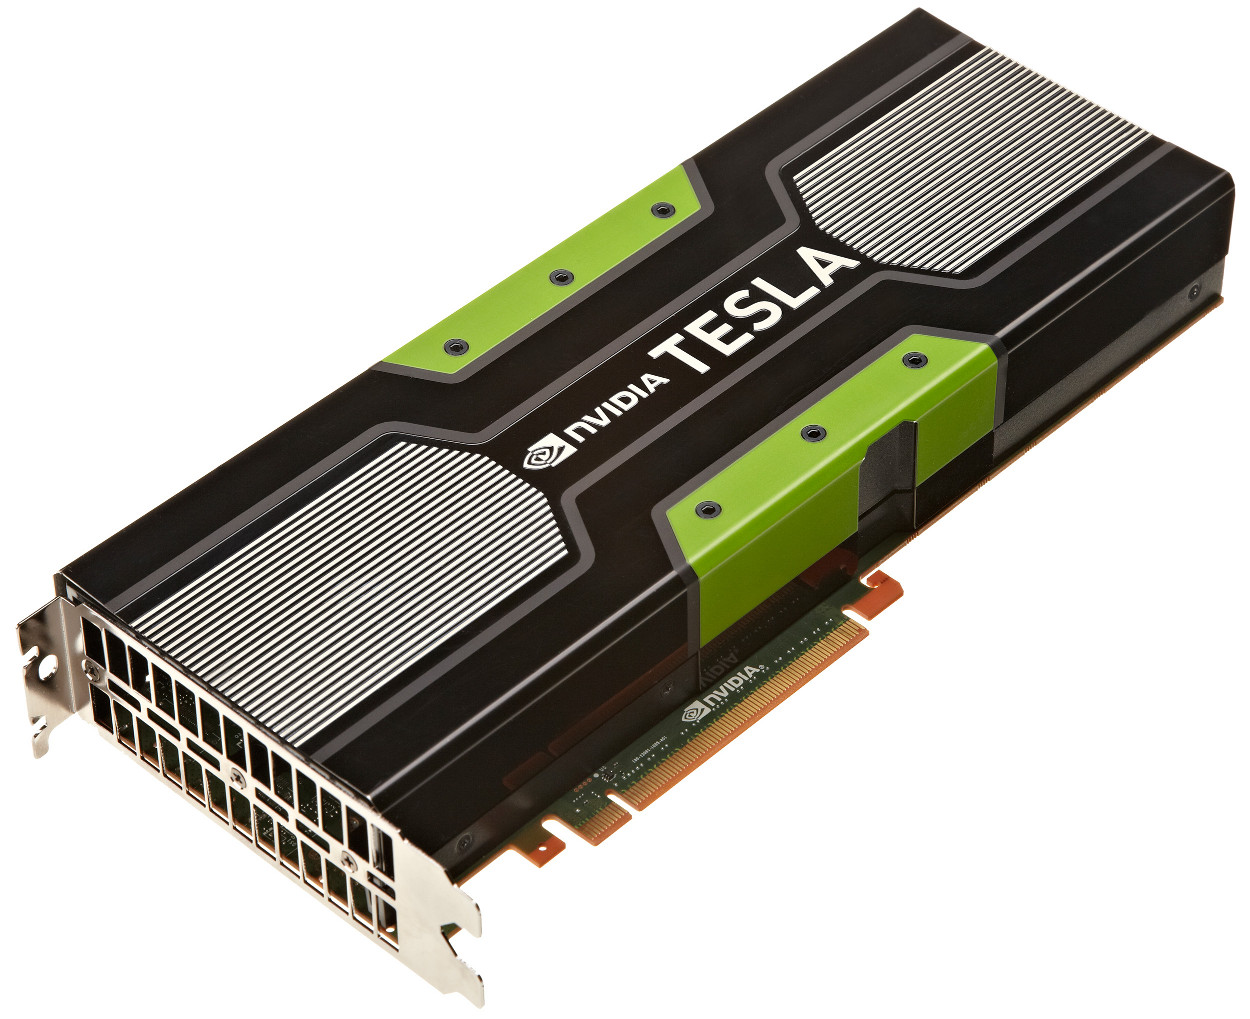
\includegraphics[width=0.7\textwidth]{figures/TeslaK20.jpg} \\ NVIDIA Tesla K20 \\ 250 (208) GB/sec
    \end{center}
   \end{minipage}


\end{frame}



\begin{frame}{Multigrid}

 \begin{block}{Programming Model}
  \begin{itemize}
   \item FirePro W9100: OpenCL
   \item Tesla K20: CUDA, OpenCL
   \item Xeon Phi: OpenCL, OpenMP
  \end{itemize}
 \end{block}

 \begin{block}{OpenCL for Everything?}
  \begin{center}
  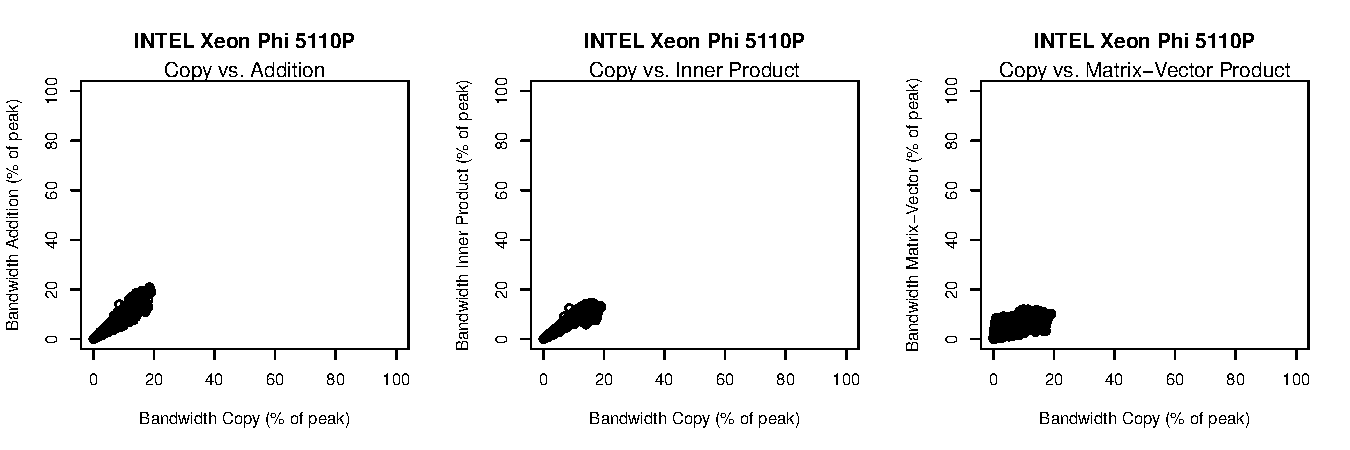
\includegraphics[width=0.99\textwidth]{figures/xeon_phi_float_xy_copy.pdf}
  \end{center}
 \end{block}

\end{frame}

\begin{frame}{Multigrid}

 \begin{minipage}{0.6\textwidth}
 \begin{block}{Ingredients of Algebraic Multigrid}
  \begin{itemize}
   \item Smoother (Relaxation schemes, etc.)
   \item Coarsening
   \item Interpolation (Inter-grid transfer)
  \end{itemize}
 \end{block}
 \end{minipage}

 \begin{minipage}{0.48\textwidth}
  \begin{center}
  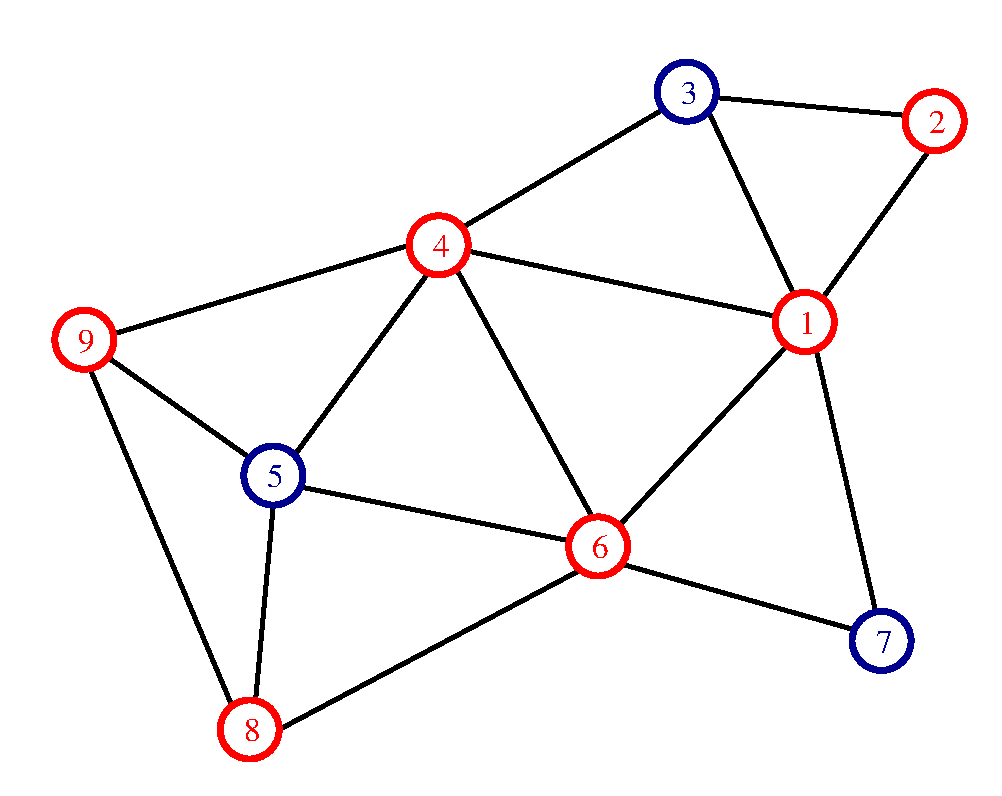
\includegraphics[width=0.99\textwidth]{figures/graph-rs.pdf} \\
    Classical coarsening
  \end{center}
 \end{minipage}
 \begin{minipage}{0.48\textwidth}
  \begin{center}
    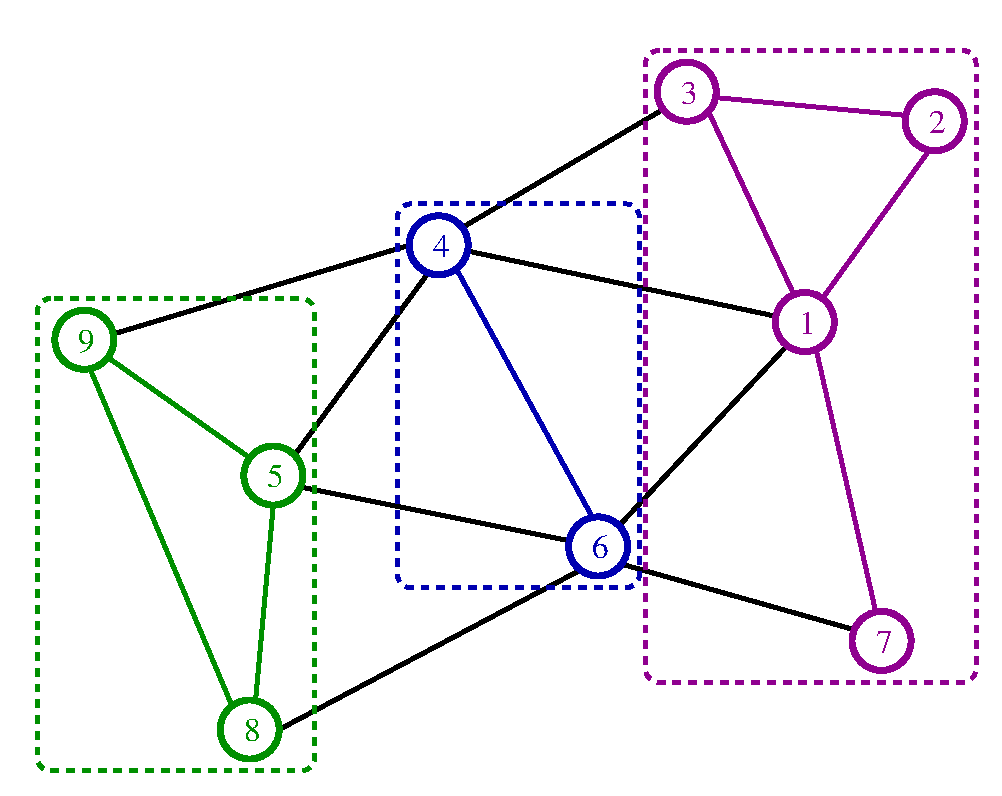
\includegraphics[width=0.99\textwidth]{figures/graph-ag.pdf} \\
    Aggregation coarsening
  \end{center}
 \end{minipage}
 \vspace*{.5cm}
\end{frame}


\begin{frame}{Multigrid Parallelization}

 \begin{block}{Setup Phase}
  \begin{itemize}
   \item Determination of coarse points in parallel by graph splitting
   \item Compute coarse operators $A^{k+1} = R^k A^k P^k$ (where $A^0 = A$)
   \item Datastructures: analyze and allocate
   \item Limited fine-grained parallelism
  \end{itemize}
 \end{block}

 \begin{minipage}{0.58\textwidth}
 \begin{block}{Cycle Phase}
  \begin{itemize}
   \item Parallel Jacobi Smoother
   \item Restriction $R^k x^k$, prolongation $P^k x^{k+1}$
   \item Direct solution on coarsest level
   \item Static datastructures
   \item Enough fine-grained parallelism
  \end{itemize}
 \end{block}
 \end{minipage}
 \begin{minipage}{0.4\textwidth} \vspace*{-1.5cm}
  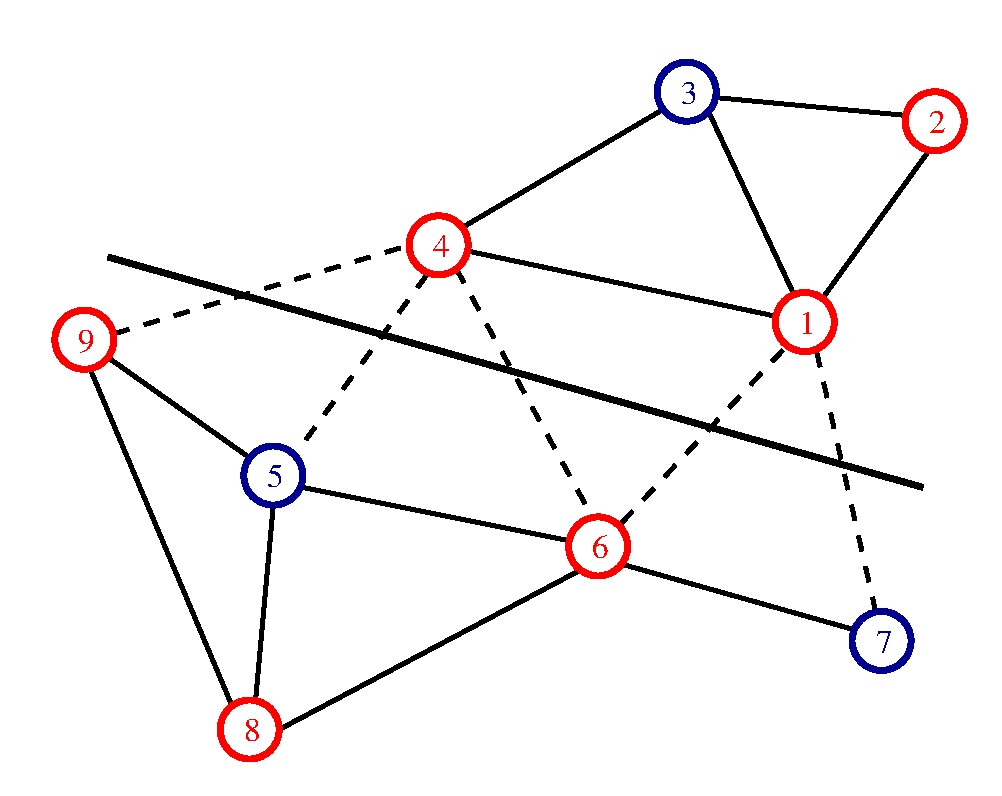
\includegraphics[width=0.99\textwidth]{figures/graph-rs0.pdf}
 \end{minipage}

 \vspace*{0.5cm}

\end{frame}



\begin{frame}{Multigrid Parallelization}

  \begin{block}{Why is AMG Hard?}
  \begin{itemize}
   \item Several thread launches with little work
   \item Sequential stages
   \item PCI-Express latency
   \item Unstructured data access
  \end{itemize}
  \end{block}

  \begin{center}
   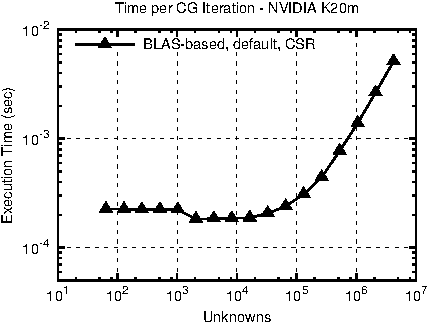
\includegraphics[width=0.5\textwidth]{figures/cg-k20m-0.pdf}
  \end{center}

\end{frame}


\begin{frame}{Scope of Comparison}

  \begin{block}{Coarsening Strategies}
  \begin{itemize}
   \item Classical One-Pass Coarsening
   \item Aggregation-based Coarsening
  \end{itemize}
  \end{block}

  \begin{block}{Interpolation Strategies}
  \begin{itemize}
   \item Direct Interpolation
   \item Aggregation-based Interpolation
  \end{itemize}
  \end{block}

  \begin{block}{Systems}
  \begin{itemize}
   \item Poisson equation in 2D, uniformly refined
   \item First-order finite elements
  \end{itemize}
  \end{block}

\end{frame}



\begin{frame}{Benchmarks}
  \begin{center}
   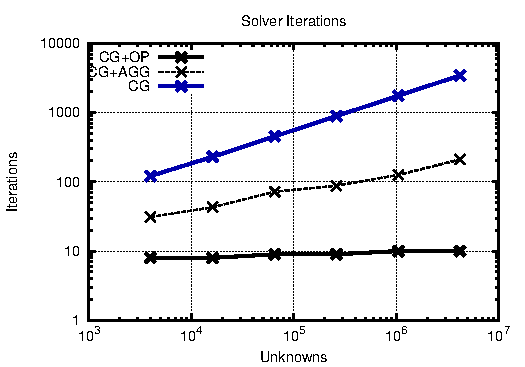
\includegraphics[width=0.99\textwidth]{figures/iters.pdf}
  \end{center}
\end{frame}


\begin{frame}{Benchmarks}
  \begin{center}
   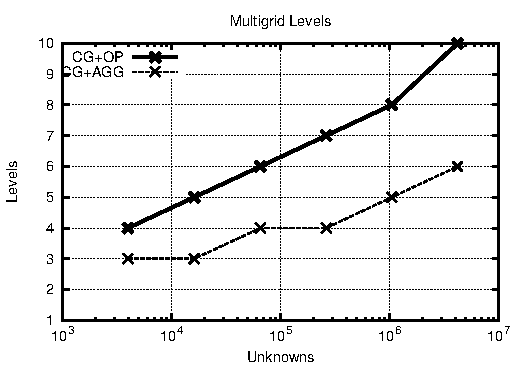
\includegraphics[width=0.99\textwidth]{figures/levels.pdf}
  \end{center}
\end{frame}

%%%%%%%%%%%%%%%%%%%%%%%%%%%%%%%%%%%%%%%%%

\begin{frame}{Benchmarks}
  \begin{center}
   2x INTEL Xeon E5-2620 v2
  \end{center}
\end{frame}
\begin{frame}{Benchmarks}
  \begin{center}
   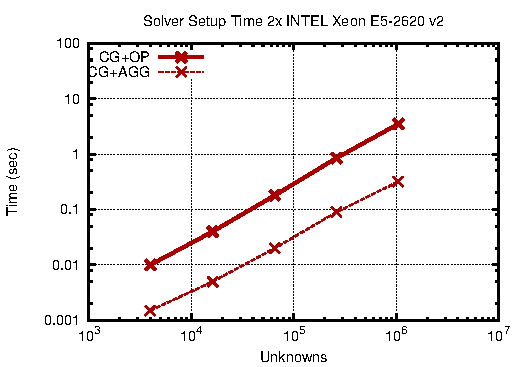
\includegraphics[width=0.99\textwidth]{figures/cpu-setup.pdf}
  \end{center}
\end{frame}
\begin{frame}{Benchmarks}
  \begin{center}
   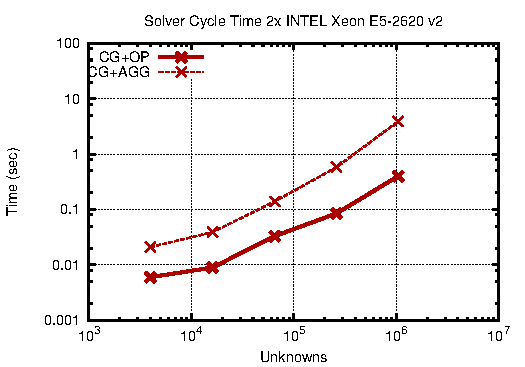
\includegraphics[width=0.99\textwidth]{figures/cpu-cycle.pdf}
  \end{center}
\end{frame}
\begin{frame}{Benchmarks}
  \begin{center}
   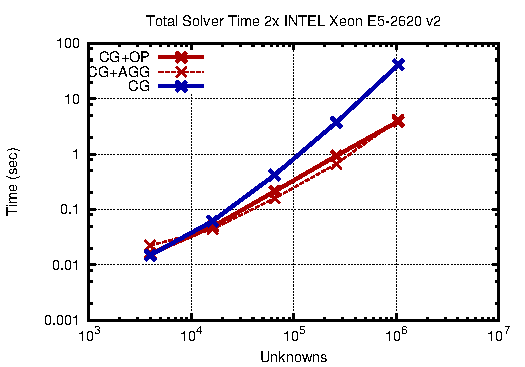
\includegraphics[width=0.99\textwidth]{figures/cpu-full.pdf}
  \end{center}
\end{frame}


\begin{frame}{Benchmarks}
  \begin{center}
   INTEL Xeon Phi
  \end{center}
\end{frame}
\begin{frame}{Benchmarks}
  \begin{center}
   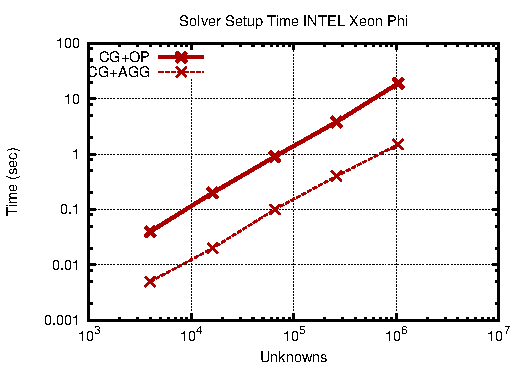
\includegraphics[width=0.99\textwidth]{figures/mic-setup.pdf}
  \end{center}
\end{frame}
\begin{frame}{Benchmarks}
  \begin{center}
   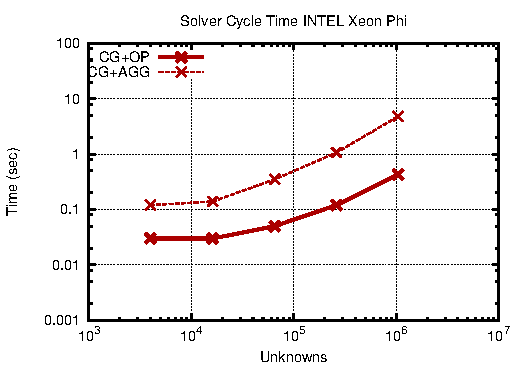
\includegraphics[width=0.99\textwidth]{figures/mic-cycle.pdf}
  \end{center}
\end{frame}
\begin{frame}{Benchmarks}
  \begin{center}
   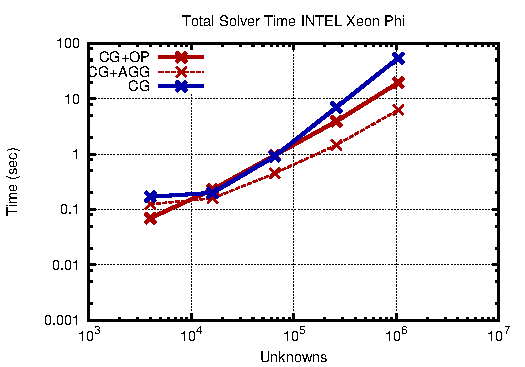
\includegraphics[width=0.99\textwidth]{figures/mic-full.pdf}
  \end{center}
\end{frame}


\begin{frame}{Benchmarks}
  \begin{center}
   NVIDIA Tesla K20
  \end{center}
\end{frame}
\begin{frame}{Benchmarks}
  \begin{center}
   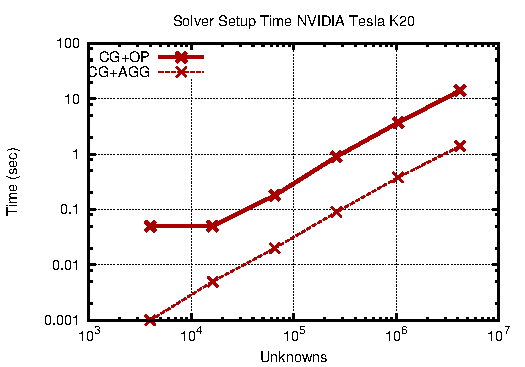
\includegraphics[width=0.99\textwidth]{figures/k20-setup.pdf}
  \end{center}
\end{frame}
\begin{frame}{Benchmarks}
  \begin{center}
   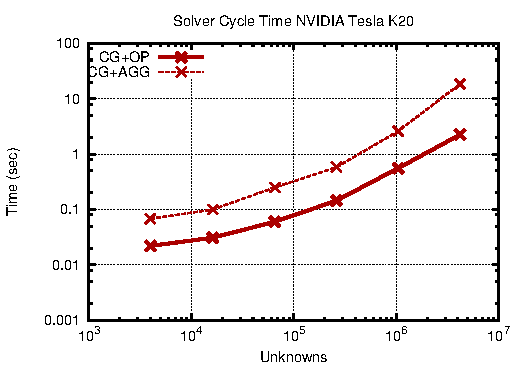
\includegraphics[width=0.99\textwidth]{figures/k20-cycle.pdf}
  \end{center}
\end{frame}
\begin{frame}{Benchmarks}
  \begin{center}
   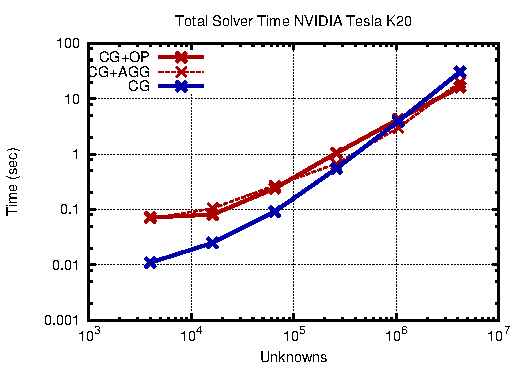
\includegraphics[width=0.99\textwidth]{figures/k20-full.pdf}
  \end{center}
\end{frame}


\begin{frame}{Benchmarks}
  \begin{center}
   AMD FirePro W9100
  \end{center}
\end{frame}
\begin{frame}{Benchmarks}
  \begin{center}
   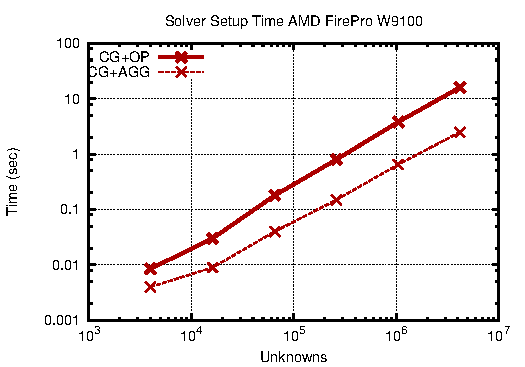
\includegraphics[width=0.99\textwidth]{figures/w9100-setup.pdf}
  \end{center}
\end{frame}
\begin{frame}{Benchmarks}
  \begin{center}
   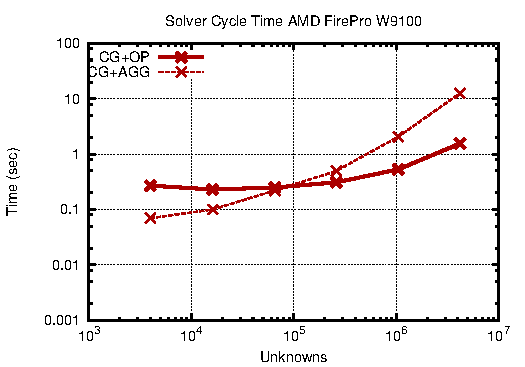
\includegraphics[width=0.99\textwidth]{figures/w9100-cycle.pdf}
  \end{center}
\end{frame}
\begin{frame}{Benchmarks}
  \begin{center}
   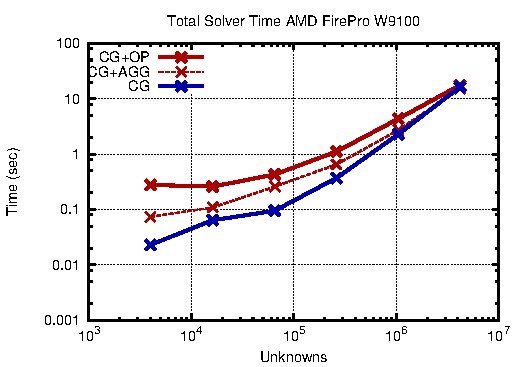
\includegraphics[width=0.99\textwidth]{figures/w9100-full.pdf}
  \end{center}
\end{frame}


%%%%%%%%%%%%%%%%%%%%%%%%%%%%%%%%%%%%%%%%%


\begin{frame}{Benchmarks}
  \begin{center}
   Putting all together...
  \end{center}
\end{frame}

\begin{frame}{Benchmarks}
  \begin{center}
   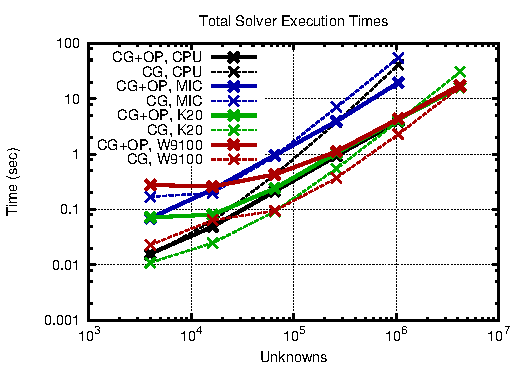
\includegraphics[width=0.99\textwidth]{figures/amg-vs-pure-full-4.pdf}
  \end{center}
\end{frame}




%%%%%%%%%%%%%%%%%%%%%%%%%%%%%%%%%%%%%%%%%

\begin{frame}{Summary and Conclusion}

  \begin{block}{Parallel AMG}
    \begin{itemize}
     \item Setup on CPU, Cycles on GPUs
     \item Sweet spot for GPUs above 1 million unknowns, below 10 million
     \item Sweet spot for MIC still to be found
    \end{itemize}
  \end{block}

  \begin{block}{Parallel Setup}
    \begin{itemize}
     \item PCI-Express and sequential stages a bottleneck
     \item Matrix transposition hard on MIC, easier on GPU
     \item Galerkin-products fastest on CPU
    \end{itemize}
  \end{block}

  \begin{block}{Availability}
  \begin{center}
   \texttt{http://viennacl.sourceforge.net/}
  \end{center}

  \end{block}

\end{frame}


%%%%%%%%%%%%%%%%%%%%%%%%%%%%%%%%%%%%%%%%%
